\chapter{Large Language Model: Theory} \label{ch:llmtheory}

This chapter serves as an overview of the large language model from the theory and technical perspective. LLM is a successful practice of NLP and beyond. It can not only process human languages but also generate new contents based on human language written requirements. The introduction of multimodal LLM further allows LLM to understand and generate not just writings but also pictures and videos.

Nowadays, it is possible for a regular user to leverage on commercialized models to develop his own applications. Given a powerful machine, a user can even deploy LLMs locally in a few steps. Open-source LLMs are available so that the user does not need to train a model from scratch. The deployment of LLMs and the interaction with them are introduced in the next Chapter \ref{ch:llmpractice}.

Modern LLMs are built on top of Transformer framework which has been introduced in earlier Chapter \ref{ch:transformer}. It is worth emphasizing the relationship between the Transformer and LLM. Transformer is an ANN framework designed for processing any sequential data so long as it can be encoded, and apparently NLP is an important use case of it. LLM is a practice of Transformer on NLP.

\section{Introduction to LLM}

This section reviews existing NLP methods and their limitations, and discusses the gaps that LLM bridges.

\subsection{Existing NLP Models and Gaps}

There have been variety of ways to model natural languages. For example, consider the following sentence:
\begin{center}
	\textit{``I am thirsty. Please give me a bottle of \rule{1cm}{0.15mm}.''}
\end{center}
It is quite natural that a human would likely to put ``water'' or ``tea'' in the blank. This is obvious because human has a dictionary of words that he can choose in his mind, and he has been reinforced of learning ``a bottle of water'' expression in many occasions. In addition, it makes sense to a human that when someone is thirsty, he would look for water.

The challenge using AI on the above task is to build the ``dictionary'' in the machine and quantitatively analyze what word or phrase would make the most sense to be filled into the blank. Many models have been proposed to solve this problem, some of which have been evolving over time in the past decades since $1990$th.

\vspace{0.1in}
\noindent \textbf{Statistical Language Models}
\vspace{0.1in}

In the early days when AI and ANN were not popular, \mync{statistical language models}[SLM] have been the most popular tool to model natural languages. SLM assumes that a sentence is a Markov process, and the last word depends on the context created by the most recent $n$ words. SLM with a fixed context length of $n$ is also called an $n$-gram language model.

Conventionally, the paring information from $n$ words to the next word is obtained from data corpus and stored in a table-like structure. When running the model, it looks up the table for the most probable next word based on the earlier $n$ words. Smoothing technologies are used to handle zeros, i.e., when the record is not found in the table.

An obvious issue of SLM is that the computation and storage of the model increase exponentially with the size of $n$. This limits the context information that the model can use for prediction, hence setting a low performance ceiling. Not to mention that even with a large data corpus, zeros can still happen and the model performance is always an issue in such occasions.

\vspace{0.1in}
\noindent \textbf{Neural Language Models}
\vspace{0.1in}

With the introduction of ANN, in particular RNN, \mync{Neural Language Models}[NLM] became popular. RNN-based NLM builds the word prediction function conditioned on the aggregated context features abstracted and passed recurrently from current and previous input sequence. More about RNN has been introduced in Chapter \ref{ch:rnn}.

RNN is not a perfect one-stop solution either. The training of RNN can be difficult due to vanishing and exploding gradient problems. This limits the depth that RNN can go. When handling long sequence of words, the performance of RNN drops significantly because it is weak at building long-term dependencies.

\vspace{0.1in}
\noindent \textbf{Pre-trained Language Models and Large Language Models}
\vspace{0.1in}

As introduced in details in earlier chapters, attention mechanism has been proposed to tackle the long-term dependency problem of RNN. Transformer architecture, which relies purely on encoder, decoder and attention mechanism without using RNN is then proposed. It has been verified that transformer architecture is good at abstracting information from sequential data, in particular, natural languages. With a transformer, it becomes possible to build very deep neural networks and have it trained efficiently with big-size data corpus. The outcome is known as the \mync{large language model}[LLM].

Language models based on different transformer-based architectures are often called \mync{Pre-trained Language Models}[PLM]. LLM can be taken as a subset of PLM. The main difference between an LLM and a regular PLM is the size of the model. The scaling of the model from hundreds of millions of parameters for PLMs to tens or hundreds of billions of parameters for LLMs introduces emergent abilities such as in-context learning to the model, significantly enhancing its capability and intelligence. As of this writing, it is not very clear how the these abilities suddenly emerge with the size of the model.

\subsection{LLM Features and Capabilities}

When the size of the model becomes large, usually to the order of at least a few billions parameters, they suddenly gain emergent abilities. Details are discussed as follows.

\vspace{0.1in}
\noindent \textbf{In-context Learning}
\vspace{0.1in}

\mync{In-Context Learning}[ICL] allows the behavior of the model to be manipulated via not training or fine-tuning of the parameters, but via instructions and demonstrations given as part of the input.

ICL plays an important part in LLM implementation, as it is the basis of prompt engineering. When the LLM is large, it is possible to use prompt engineering instead of fine-tuning to complete a task following user defined instructions. This reduces the training cost and makes the implementation more flexible.

\vspace{0.1in}
\noindent \textbf{Instruction Following}
\vspace{0.1in}

Supervised learning is commonly used in training and fine-tuning a model. In the training set, we need to provide the model ``examples''. An example includes the input, some good responses, and some bad responses. 

When comes to LLM, it is possible to fine-tune a model for a specific task without using the aforementioned examples. Instead, just give it step-by-step instructions. LLM is able to perform well with these tasks described only by instructions. This is known as instruction tuning.

It is worth mentioning that instruction following is also possible in ICL. Give the LLM instructions in prompt engineering without examples, and the LLM is likely to be able to finish the tasks.

\vspace{0.1in}
\noindent \textbf{Step-By-Step Reasoning}
\vspace{0.1in}

When a model is asked to complete a complicated task that involves multiple steps, it may fail to accomplish the task. With a well fine-tuned LLM, the model might be able to break the task into multiple sub-tasks via \myabb{chain-of-thought}{CoT} prompting strategy, and solve them step-by-step till the final result is obtained.

It has been observed that an LLM with at least $100B$ parameters is likely to have good step-by-step reasoning abilities.

The performance of an LLM, usually referring to its capability in accurately and correctly complete a task, is affect by many factors such as the model architecture, model size, training data set size and quality, etc. Though it is clear that with the scaling up of the system the performance is usually improved, there is no analytical expression that gives full insights about how these factors affect the performance quantitatively.

A \mync{scaling law} tries to quantitatively describe the performance of an LLM as a function of model size and other factors. Many scaling laws have been proposed, many of which obtained from empirical experiments and they may work only within a given range of model size.

Just as an example, OpenAI proposed KM scaling law in 2020 that describes LLM cross entropy loss as a function of model size, training data set size and training computation as follows.
\begin{eqnarray}
	L(N) &=& \left(\dfrac{N_c}{N}\right)^{\alpha_N} \nonumber \\
	L(D) &=& \left(\dfrac{D_c}{D}\right)^{\alpha_D} \nonumber \\
	L(C) &=& \left(\dfrac{C_c}{C}\right)^{\alpha_C} \nonumber
\end{eqnarray}
where $N$, $D$ and $C$ denote the model size, dataset size and training computation, respectively. The rests are constants whose value can be obtained via calibration.

This scaling law works for models with $22M$ to $23B$ parameters. It is assumed that the analysis of a factor can be done independently without other parameters being a bottleneck.

\subsection{LLM Performing Benchmarks}

\subsection{LLM Development Timeline}

A brief timeline of the development of LLMs since the publication of \cite{vaswani2017attention} is given below.

\vspace{0.1in}
\noindent \textbf{2017}
\vspace{0.1in}

``Attention Is All You Need'' \cite{vaswani2017attention} introduced a new type of NLP model called the ``Transformer''. Unlike traditional RNN-based models, the Transformer removes all recurrent components and adopts an encoder-decoder architecture that relies entirely on self-attention mechanisms to model dependencies within and across sequences.

\vspace{0.1in}
\noindent \textbf{2018-2020}
\vspace{0.1in}

OpenAI released the GPT-1, GPT-2, and GPT-3 models in consecutive years from 2018 to 2020, showcasing the scalability of Transformer-based architectures for autoregressive language modeling.

\vspace{0.1in}
\noindent \textbf{2022}
\vspace{0.1in}

\myabb{Reinforcement Learning from Human Feedback}{RLHF} became a widely adopted training strategy. OpenAI released ChatGPT, a chatbot fine-tuned from the GPT-3.5 model using RLHF. Its human-like conversational abilities captured public attention and spurred a surge of interest and development in LLM-based applications.

\vspace{0.1in}
\noindent \textbf{2023-2024}
\vspace{0.1in}

GPT-4, GPT-4o are published in 2023 and 2024 respectively, along with many other frontier models are published.

\subsection{LLM-Relevant Milestone Technologies}

This section looks back into the progression tree of LLM, and lists down milestone techniques that make LLM what it is today. It is the breakthrough in these areas that revolutionizes LLM development.

\vspace{0.1in}
\noindent \textbf{Big Data}
\vspace{0.1in}

The performance of LLM relies on both the modal size and the training data size. It is the advent in internet, Web 3.0, Industry 4.0, IoT and cloud computing/storage that makes collection and aggregation of big data possible.

Almost every large-size enterprise, both IT companies and conventional industrial companies, have their internal databases. The database can be used to train domain-knowledge LLM. Nowadays, there are many open data sources of community LLMs. Such examples include BookCorpus, CommonCrawl, Reddit posts (with high upvotes), Wikipedia, and many more. These open-source datasets make training LLM for community projects possible.

\vspace{0.1in}
\noindent \textbf{Large Model and Efficient Training}
\vspace{0.1in}

The invention of CPU-based neural networks and transformer architecture making creating and training large scale LLM possible. Both closed and open-source LLMs have been proposed, including GPT series by OpenAI and LLaMA family by Meta AI and the community.

Manly libraries have been released to the public to help building, training and fine-tuning LLMs, such as \verb|transformers|, a Python library for building transformer models. Many such libraries are tying up with PyTorch and TensorFlow to provide LLM related functions.

More about these models and libraries are introduced in later sections.

\vspace{0.1in}
\noindent \textbf{Fine-Tuning}
\vspace{0.1in}

Technologies such as LoRA has made fine-tuning easier than before.

\vspace{0.1in}
\noindent \textbf{Prompt Engineering}
\vspace{0.1in}

There have been a lot of practices on how to make LLM flexible and more efficient in solving particular tasks via prompt engineering.

\vspace{0.1in}
\noindent \textbf{LLM on Edge Devices}
\vspace{0.1in}

Many efforts have been put into edge-device based LLMs. The target is to develop LLM that consumes less memory, storage and computation while not sacrificing a lot of performance.

\vspace{0.1in}
\noindent \textbf{API and Interface}
\vspace{0.1in}

Multi-modal LLM has enabled different types of inputs to the LLM, not limited to natural language but also sequential signals and even pictures.

Many tools and software have developed APIs for LLM. These tools enhance computation and online information retrieval capabilities of LLM.

\section{Existing LLMs Features}

As of this writing, there are countless LLMs available on the market or within the open-source community, and the list continues to evolve rapidly. 

This section introduces the shared properties and general characteristics of existing LLMs, without delving into detailed performance metrics or task-specific comparisons. The goal here is not to promote one model over another, but rather to provide a broad overview of what defines an LLM in practice.

A more detailed performance review of selected models is provided in Section~\ref{sec:frontierllmmodels}.


Many LLMs are capable of engaging in human-like conversations and answering questions in depth. Some can even search the internet for the up-to-date relevant information to support their responses. Most well-known LLMs can also follow user instructions to perform specific tasks, such as completing a piece of code, provided the prompts are sufficiently clear and aligned with the model's training data.

That said, many LLMs (unless specifically trained on domain-specific corpora) do not perform as well as experienced professionals in specialized fields. It is often claimed that top-performing LLMs can achieve a level of performance comparable to fresh PhD graduates in certain tasks, although a noticeable gap remains when compared to experienced researchers.

LLMs may generate inaccurate or misleading information while expressing it in a fluent and confident manner. This behavior stems from the their lack of self-awareness and inability to judge the factual correctness of its outputs.

LLMs can also struggle with detailed quantitative tasks. This limitation arises from how they process and generate language: input is tokenized into subword or word-like units, and outputs are generated based on statistical patterns rather than precise symbolic reasoning. For example, an LLM might fail to correctly answer a seemingly simple question like ``How many letters `a' are there in this sentence?'', because its training does not emphasize accurate character-level counting.

Multimodal LLMs can generate images or videos based on textual descriptions. However, they often struggle to accurately render fine-grained visual details. For example, if prompted to generate an image of a car with a license plate that reads ``3.14159265358979'', the resulting image may omit or distort some of the digits. This limitation stems from the fact that image generation is driven by probabilistic pattern synthesis, not precise symbolic encoding or controlled rendering of visual elements. An example is given in Fig. \ref{fig:gpt_carplate}.

\begin{figure}[!htb]
	\centering
	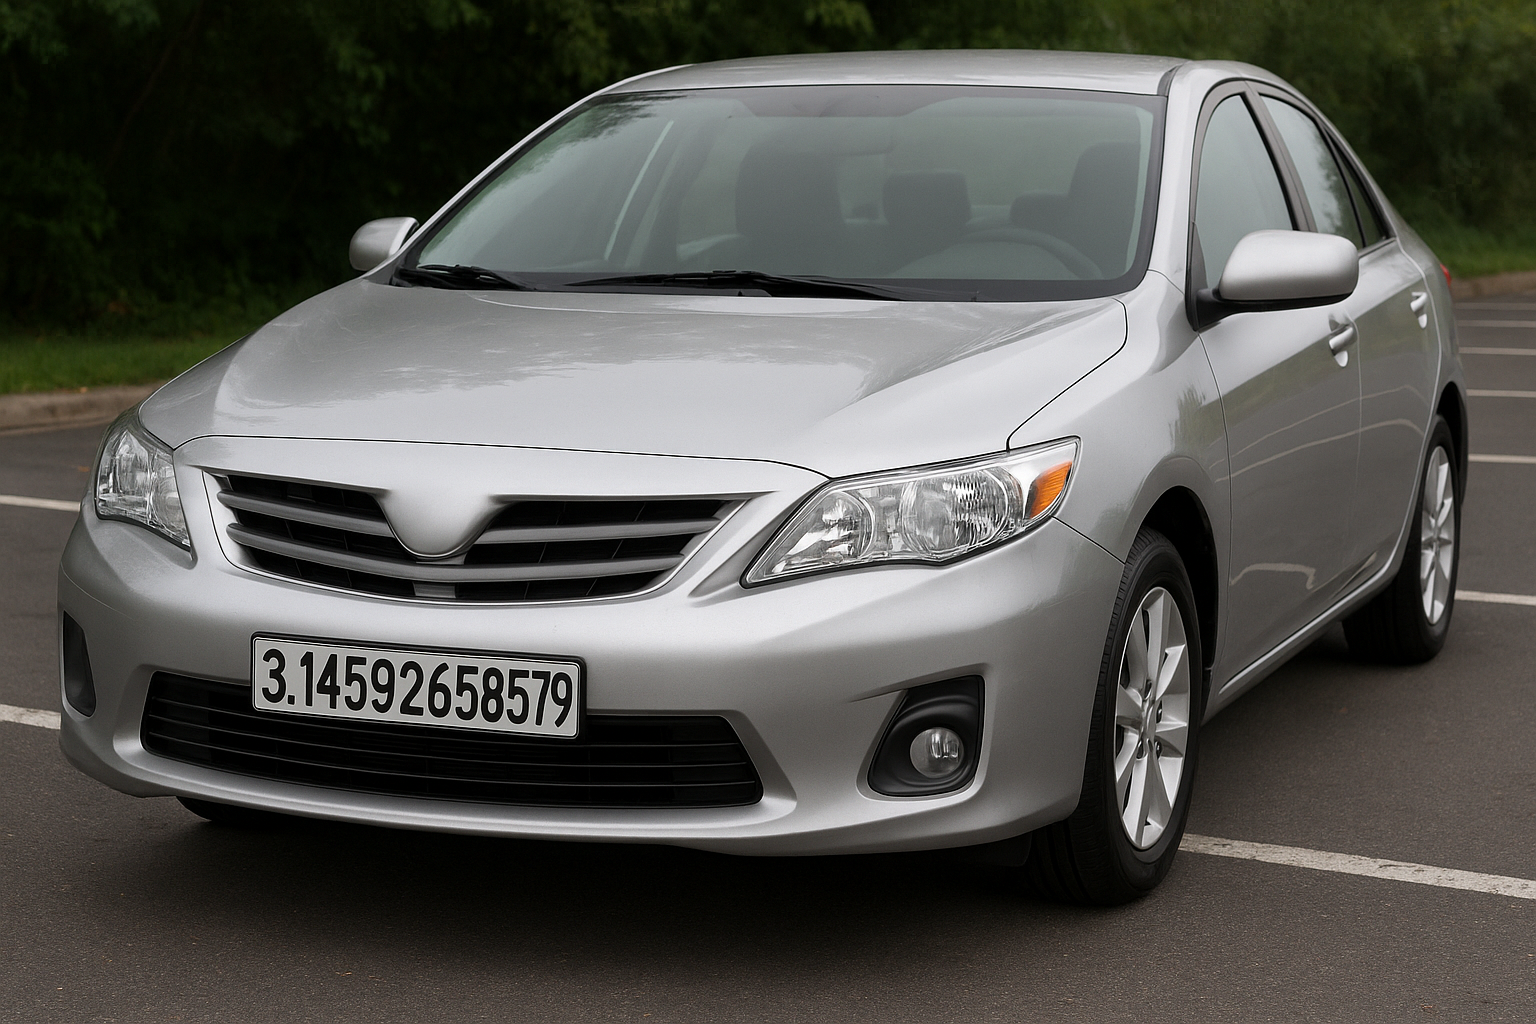
\includegraphics[width=0.5\textwidth]{./chapters/part-7/figures/gpt_carplate.png}
	\caption{A figure from a GPT when it is asked to generate a car with a license plate that reads ``3.14159265358979''.}
	\label{fig:gpt_carplate}
\end{figure}

It is true that each LLM is trained and fine-tuned with different data corpus and may behave differently on different types of tasks. Consider LLMs with the same model structure and training strategy. In such case, models with larger training data sets and more parameters often outperform those with smaller training data sets and less parameters. From application perspective, the trend is that the frontier models' performances are converging for regular tasks, and the costs are going to be the main differentiator. 

OpenAI's GPT models and Meta's LLaMA models are the first models that gain popularity. A brief review is given in the remaining of the section.

\subsection{OpenAI Family}

OpenAI started investigating language models before the proposition of transformer. In its early days, RNN was explored as the most promising model for natural language. In 2017 when the transformer model was proposed, OpenAI quickly adapted their language model to this new architecture, and as a result generative pre-training (GPT) series has been proposed.

\vspace{0.1in}
\noindent \textbf{GPT-1}
\vspace{0.1in}

GPT-1, OpenAI's first transformer based PLM was proposed in 2018. GPT-1 has $117M$ parameters in the model and it adopts a decoder-only architecture, which is different from the original transformer proposal which has a encoder-decoder architecture. GPT-1 was trained via a two-stage procedure, the first stage unsupervised pre-training and the second stage supervised fine-tuning. This two-stage training pipeline, or something of the similar kind, has been adopted by many LLMs coming after.

\vspace{0.1in}
\noindent \textbf{GPT-2}
\vspace{0.1in}

GPT-2 is an improvement of GPT-1. It uses much larger number of parameters of $1.5B$ in the model, and it was trained on a much larger dataset WebText. With larger model and training data size, GPT-2 is targeted to be a multi-task solver. The model can be formulated by the following probabilistic form
\begin{eqnarray}
  \textup{Pre-trained LLM} &\equiv& P\left(\textup{output}\middle|\textup{input}, \textup{task}\right) \nonumber
\end{eqnarray}
In the above formulation, each NLP task can be considered as the word prediction problem based on a subset of the word next, and can be trained during the unsupervised learning stage. Unsupervised pre-training has since then become the most important stage for the LLM to gain knowledge for general tasks.

\vspace{0.1in}
\noindent \textbf{GPT-3, GPT-3.5 and Chat-GPT}
\vspace{0.1in}

It is clear now that GPT-2 has $1.5B$ parameters which is too few for an LLM to gain emergent abilities. It is GPT-3 with $175B$ parameters trained on $300B$ tokens that made a capability leap and bring LLM to everyone's attention.

It is GPT-3 that for the first time introduces emergent abilities such as ICL. GPT-3 not only accomplishes commonly seen tasks to test LLM capabilities with flying color, but also demonstrates features not shown by other models before, such as reasoning and domain adaption.

OpenAI has developed many task-oriented models that use GPT-3 as the base model. For example, for coding, Codex was introduced. Codex is basically GPT-3 fine-tuned using code database such as GitHub. Comparing with GPT-3, Codex is able to reason and solve complex mathematical problems, and realize them in codes. RL had already been used to fine-tune and improve performance for GPT-2. The same has been applied on GPT-3. Furthermore, reinforcement learning with human feedback (RLHF) is introduced for GPT-3 that allows the model to continue learning from human demonstrations.

With the above enhancements, i.e. code-based fine-tuning, RL and RLHF, GPT-3.5 has been developed. GPT-3.5 is an enhanced version of GPT-3 and it is obtained from GPT-3 via transfer learning. GPT-3.5 is also scaled up in size, with a parameter number of $335B$.

Chat-GPT was developed on top of GPT-3.5 (and later another version was released developed on top of with GPT-4). It is GPT-3.5 fine-tuned specially optimized for dialogue. It demonstrates how LLM can be used in everyone's daily life as an assistant, consultant and a copilot. Chat-GPT demonstrated good performance in communicating of humans than other GPT models. This is because Chat-GPT is trained on human-generated conversations of both human and AI roles. Later on, plug-ins and APIs are enabled on Chat-GPT, to allow it to communicate with other software.

\vspace{0.1in}
\noindent \textbf{GPT-4}
\vspace{0.1in}

GPT-4 is a multimodal LLM, meaning that it can not only take in natural languages, but also other signals such as images. Comparing with GPT-3.5, GPT-4 demonstrates further enhanced capabilities. It is claimed that GPT-4 is safer to use and is less likely to generate toxic and misleading information.

Just as a quick demonstration of its multimodal feature, pass the following Fig. \ref{fig:superpower_cat} (notice that this figure itself is generated by an AI model) to GPT-4 with instruction ``What is in this picture?''. GPT-4 is able to response the following:

\vspace{0.1in}
\noindent \textit{``The image showcases a majestic cat standing in a fantastical landscape. The cat emits a luminous, ethereal glow, and its fur and tail appear to be infused with swirling, fiery or cosmic energies in brilliant hues of red and gold. These radiant swirls surround the cat, adding to its supernatural aura. Behind the cat, there's a dramatic night sky with clouds illuminated by a hidden light source, possibly lightning or a celestial event. In the foreground, the terrain appears to be a combination of grassy knolls and fiery, ember-lit ground, further emphasizing the magical and otherworldly nature of the scene. The entire setting evokes a sense of wonder and fantasy.''}
\vspace{0.1in}

\begin{figure}[!htb]
	\centering
	
\includegraphics[width=0.6\textwidth]{./chapters/part-7/figures/superpower_cat.png}
	\caption{A cat with superpower. This picture is generated by DALL$\cdot$E 3.}
	\label{fig:superpower_cat}
\end{figure}

\vspace{0.1in}
\noindent \textbf{Other OpenAI Models}
\vspace{0.1in}

DALL$\cdot$E is the model OpenAI uses to generate images. As of this writing, its latest version, DALL$\cdot$E 3, has been integrated with the latest ChatGPT. Figure \ref{fig:superpower_cat} gives an example where DALL$\cdot$E 3 is used to generate a image of a superpower cat.

OpenAI Codex, as introduced earlier, is the GPT model optimized for code generation. As of this writing, Codex has been deprecated because its capability has been integrated into ChatGPT. It is possible to ask ChatGPT to generate a piece of code following user's instruction and description.

OpenAI Codex is the engine that powers GitHub copilot. In this sense, OpenAI Codex remains a live in a different format: not as a standalone software or model, but more as an API.

\subsection{LLaMA Family}

Large Language Model Meta AI (LLaMA) is the LLM model developed by Meta AI. Different from most of the AI models (GPT-3 and onward) developed by OpenAI, LLaMA is open-source hence has a wide availability. Many efforts in the community have made modifications and improvements to LLaMA, making a big family of models with different characteristics.

As of this writing, a family tree of LLaMA is shown in Figure \ref{fig:llama_family_tree}. The picture is from \cite{zhao2023survey}. The source of the picture is given in the GitHub repository of the paper.
\begin{figure}[!htb]
	\centering
	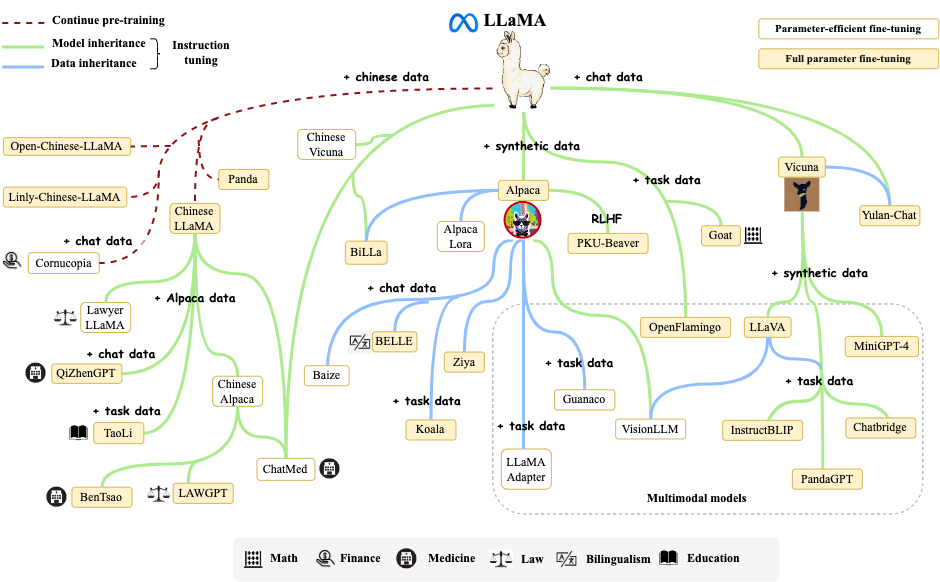
\includegraphics[width=\textwidth]{./chapters/part-7/figures/lamma_family_tree.png}
	\caption{LLaMA family tree.}
	\label{fig:llama_family_tree}
\end{figure}
Only a small portion of models in the family tree is briefly introduced here.

\vspace{0.1in}
\noindent \textbf{LLaMA}
\vspace{0.1in}

LLaMA, comparing with GPT-3 which was used as a benchmark, is smaller in model size (maximum $65B$ parameters VS $175B$ parameters in GPT-3) but larger and better in training data size and quality (maximum $1.4T$ tokens VS $300B$ tokens in GPT-3). As a result, LLaMA is able to achieve generally better performance than GPT-3 with less implementation cost due to the small size. LLaMA demonstrates that training data is equality important as model size. It is possible to reach the same level of performance with a small ($<100B$ parameters) but well-trained model.

LLaMA's first release includes 4 models of different model and training sizes. Details are summarized in Table \ref{ch:llm:tab:llamamodels}.
\begin{table}[!htb]
	\centering \caption{LLaMA models.}\label{ch:llm:tab:llamamodels}
	\begin{tabular}{ccc}
		\hline
		Name & Model Size & Training Dataset Size \\ \hline
		LLaMA 7B & $6.7B$ & $1T$ \\
		LLaMA 13B & $13.0B$ & $1T$ \\
		LLaMA 33B & $32.5B$ & $1.4T$ \\
		LLaMA 65B & $65.2B$ & $1.4T$ \\
		\hline
	\end{tabular}
	\begin{flushleft}
		\footnotesize
		Model size is given in number of parameters in billion. Training data size is given in number of tokens.
	\end{flushleft}
\end{table}
The training dataset is purely open-source, including Common Crawl, C4 Dataset, GitHub, Wikipedia, public domain books, arXiv and Stack Exchange.

Technical wise, LLaMA has some innovations on top of the original transformer proposition \cite{vaswani2017attention} n the normalization method, activation function, and embedding methods. More details will be introduced in later sections.

Many open-source tools and packages have been developed to fine-tune LLaMA and its variations. More about fine-tuning, such as LoRA\cite{hu2021lora} and QLoRA\cite{dettmers2023qlora}, are introduced in more details in later sections. Notice that fine-tuning or re-training of a model often cost a lot of computational power and vector memory.

\vspace{0.1in}
\noindent \textbf{Stanford Alpaca}
\vspace{0.1in}

Stanford Alpaca 7B is Standford's practice in fine-tuning LLaMA 7B. The running cost of this fine-tuning is impressively small (hundreds of USD), and the resulted model has a performance comparable with GPT-3.5 which has $335B$ parameters. It is impressive to see that a small $7B$ model can compete with a large $335B$ model by careful training and fine-tuning. This might be partially because Alpaca 7B is fine-tuned from LLaMA 7B using knowledge distillation from GPT-3.5 (also known as text-davinci-003).

The details of training Stanford Alpaca can be found in \cite{alpaca}. A brief highlight is given below. The fine-tuning pipeline of Alpaca is shown in Fig. \ref{fig:alpaca_pipeline}. It is a 2-stage process as follows.
\begin{enumerate}
	\item Generating instruction-following examples using GPT-3.5 (text-davinci-003).
	\item Fine-tune LLaMA 7B using the examples.
\end{enumerate}
\begin{figure}[!htb]
	\centering
	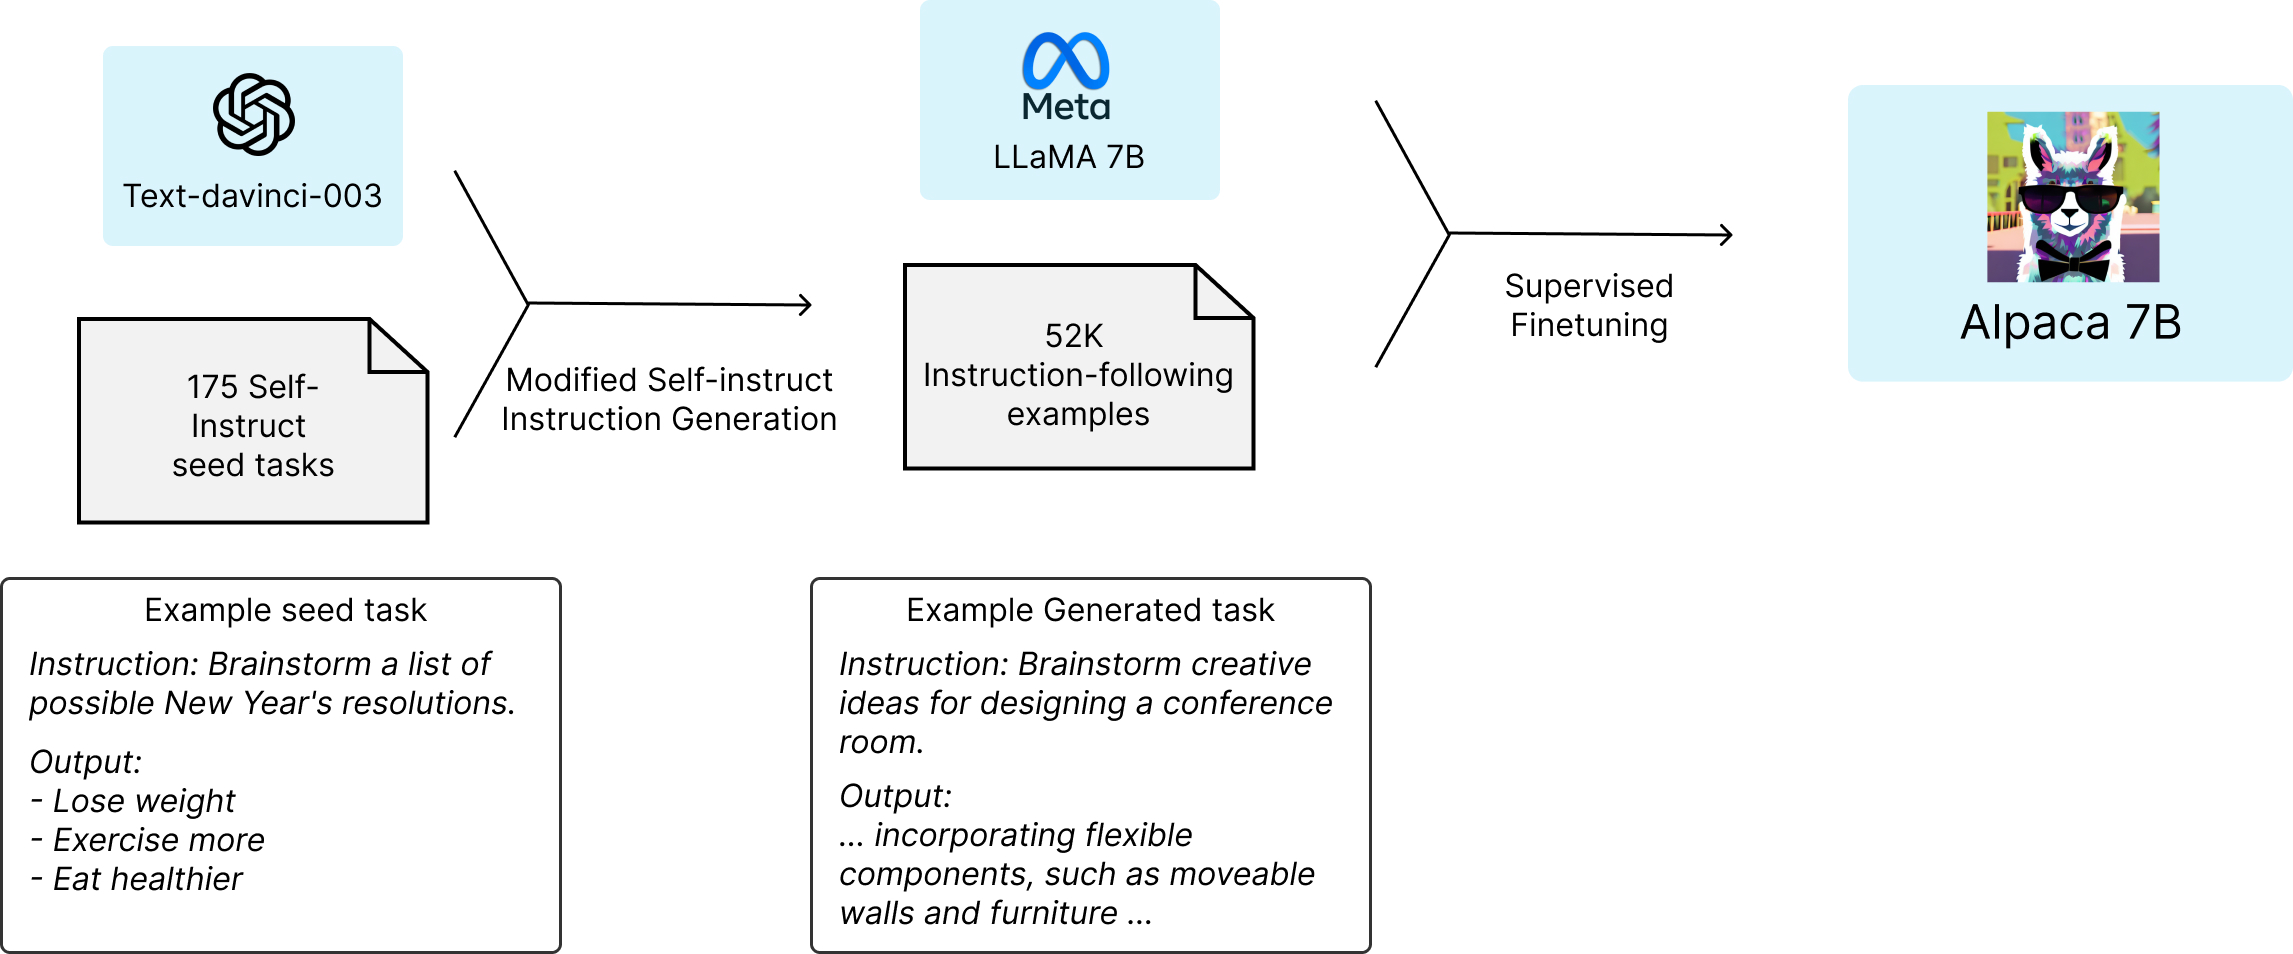
\includegraphics[width=\textwidth]{./chapters/part-7/figures/alpaca_pipeline.jpg}
	\caption{Alpaca fine-tuning pipeline.}
	\label{fig:alpaca_pipeline}
\end{figure}

Examples of the generated instruction and response pairs are given below. The full list is available from the GitHub repository.
\begin{lstlisting}
{
	"instruction": "What are the three primary colors?",
	"input": "",
	"output": "The three primary colors are red, blue, and yellow."
},
{
	"instruction": "Give three tips for staying healthy.",
	"input": "",
	"output": "1.Eat a balanced diet and make sure to include plenty of fruits and vegetables. \n2. Exercise regularly to keep your body active and strong. \n3. Get enough sleep and maintain a consistent sleep schedule."
},
{
	"instruction": "Extract the facts from the paragraph.",
	"input": "Online education continues to become more popular for schools and students alike. Its advantages are generally lower costs, less commitment and the ability to study at a time, place and pace that suits the student.",
	"output": "- Online education is becoming increasingly popular.\n- It has several advantages such as lower costs, less commitment and the ability to study at one\u2019s own time and pace."
},
{
	"instruction": "Arrange the given numbers in ascending order.",
	"input": "2, 4, 0, 8, 3",
	"output": "0, 2, 3, 4, 8"
}
\end{lstlisting}

The fine-tuning code of Alpaca is from Hugging Face. Python packages such as \verb|numpy|, \verb|torch|, \verb|transformers|, etc., are required. Check \verb|requirements.txt| and \verb|train.py| in the repository for more details. Call \verb|train.py| using something like the following
\begin{lstlisting}
torchrun --nproc_per_node=4 --master_port=<your_random_port> train.py \
	--model_name_or_path <your_path_to_hf_converted_llama_ckpt_and_tokenizer> \
	--data_path ./alpaca_data.json \
	--bf16 True \
	--output_dir <your_output_dir> \
	--num_train_epochs 3 \
	--per_device_train_batch_size 4 \
	--per_device_eval_batch_size 4 \
	--gradient_accumulation_steps 8 \
	--evaluation_strategy "no" \
	--save_strategy "steps" \
	--save_steps 2000 \
	--save_total_limit 1 \
	--learning_rate 2e-5 \
	--weight_decay 0. \
	--warmup_ratio 0.03 \
	--lr_scheduler_type "cosine" \
	--logging_steps 1 \
	--fsdp "full_shard auto_wrap" \
	--fsdp_transformer_layer_cls_to_wrap 'LlamaDecoderLayer' \
	--tf32 True
\end{lstlisting}
where \verb|./alpaca_data.json| is the JSON file that contains all the instruction and response pairs.

Notice that later on, Stanford Alpaca 13B is also developed based on LLaMA 13B.

\vspace{0.1in}
\noindent \textbf{Vicuna}
\vspace{0.1in}

Vicuna 13B is an open-source chatbot fine-tuned on top of LLaMA using $70K$ user-shared conversations collected from ShareGPT (a platform where users share their ChatGPT conversation histories). Its performance is comparable with GPT-3.5 and Bard, and it is slightly better than LLaMA 13B and Alpaca 13B in general.

See \cite{vicuna2023} for more details.

\vspace{0.1in}
\noindent \textbf{LLaVA and MiniGPT-4}
\vspace{0.1in}

Large Language and Vision Assistant (LLaVA) is a multimodal LLM that combines a vision encoder and Vicuna for general purpose visual and language understanding. More details are given in \cite{liu2023llava} and \cite{liu2023improvedllava}. Similar with GPT-4, its multimodal encoders allows it take both natural language and image as inputs. An example is given below.

Pass the same Fig. \ref{fig:superpower_cat} to LLaVA with the same instruction ``What is in this picture?''. LLaVA is able to give the following response:

\vspace{0.1in}
\noindent \textit{``The image features a cat standing on a hill, with a fiery background and a cloudy sky. The cat appears to be looking at the viewer, and there is a sense of motion in the scene.''}
\vspace{0.1in}

Similar with LLaVA, MiniGPT-4 is a also multimodal LLM that enhances vision interpretation. More details are given in \cite{zhu2023minigpt}. It uses different techniques and realizations from LLaVA. Pass the same Fig. \ref{fig:superpower_cat} to MiniGPT-4 with the same instruction ``What is in this picture?''. MiniGPT-4 is able to give the following response:

\vspace{0.1in}
\noindent \textit{``The image shows a white cat with flames coming out of its fur, standing on a hill at sunset. The cat’s eyes are closed, and it appears to be in a meditative state. The background is a dark sky with clouds and a full moon. The overall mood of the image is peaceful and mystical.''}
\vspace{0.1in}

Notice that both LLaVA and MiniGPT-4 model can be downloaded from their GitHub and HuggingFace repositories. As of this writing, live demos are also available for these models.

Multimodal LLM and ``Any-to-Any'' LLM are not the main forecast of this chapter. More details will be introduced in later chapters.

\vspace{0.1in}
\noindent \textbf{LLaMA 2}
\vspace{0.1in}

LLaMA 2 is the next generation open source LLM following the original LLaMA. The model is free for research and commercial use. LLaMA 2 70B has $70B$ parameters and it is pre-trained with $2T$ tokens of training data.

\subsection{Other LLMs}

\section{LLM Development}

This section introduces the basic steps in the LLM development workflow, should the user want to develop an LLM from scratch.

\subsection{Architecture Design}

\vspace{0.1in}
\noindent \textbf{Encoder and Decoder}
\vspace{0.1in}

\vspace{0.1in}
\noindent \textbf{Normalization Method}
\vspace{0.1in}

\vspace{0.1in}
\noindent \textbf{Activation Function}
\vspace{0.1in}

\vspace{0.1in}
\noindent \textbf{Position Embedding Method}
\vspace{0.1in}

\vspace{0.1in}
\noindent \textbf{Attention Mechanism}
\vspace{0.1in}

\subsection{Training Corpus Preparation}

Data corpus is available online for LLM training. Many libraries such as PyTorch compatible Python packages have been developed to automate the training procedures and to convenient the users.

The existing resources and solutions are briefly introduced in this section.

\subsection{Pre-training}

\subsection{Fine-Tuning}

\subsection{Model Evaluation}

\section{Multimodal LLM}

TBA

